\documentclass{article}

\author{Mathias Magnusson}
\title{Lè gÿmñæŝíéàrḃêtë}
\date{}

\usepackage{graphicx}
\usepackage{xcolor}
\usepackage{minted}
\usepackage{listings}
\definecolor{codebg}{rgb}{0.97,0.97,0.97}

\renewcommand*\contentsname{Innehållsförteckning}
\renewcommand*\listfigurename{Bilder}
\renewcommand*\listoflistingscaption{Kodavsnitt}

\renewcommand*\listingscaption{Kodavsnitt}
\renewcommand*\figurename{Bilaga}

\newcommand*\coderef[1]{\listingscaption~\ref{#1}}

\usepackage[
	pdfborder={0 0 0},
	colorlinks=true,
	linkcolor=black,
	urlcolor=blue
]{hyperref}

\makeatletter
\renewcommand*\paragraph{\@startsection{paragraph}{4}{\z@}%
			{-2.5ex\@plus -1ex \@minus -.25ex}%
			{1.25ex \@plus .25ex}%
			{\normalfont\normalsize\bfseries}}
\makeatother
\setcounter{secnumdepth}{4}
\setcounter{tocdepth}{4}

\begin{document}

\maketitle{}

\section*{Abstract}

\begin{par}

\itshape
This report describes methods used to execute untrusted code in a safe
environment. This is then used to describe an implementation of a judge system
that automates the process of continually receiving users' programs accompanied
by data describing an exercise in problem solving, and then evaluating the
program's correctness. Additionally, a web application and server is created to
serve as an interface between users and this judge, as well as storing
information about available problems and registered users.

The majority of this report describes how all of the above was, and can be,
implemented. Both text describing all methods used, as well as code snippets and
commands showing parts the actual implementation is included.

The main focus of the report lies on executing untrusted code. Less focus lies
on the web application and server, but it is still included and roughly
described.

\end{par}

\clearpage

\tableofcontents

\clearpage

\section{Inledning}

\subsection{Syfte}

Syftet med detta gymnasiearbete är att skapa en webbsida där användaren ska
kunna öva på programmeringsproblemlösning och därmed få en förståelse för hur
en säker webbserver skapas samt hur opålitlig kod kan exekveras på ett säkert
sätt.

\subsection{Bakgrund}

Den första kända tävlingen inom programmeringsproblemlösning kallades ``First
Annual Texas Collegiate Programming Championship'' (Competitive Programming,
Wikipedia) och anordnades vid ``Texas A\&M University''. Då skrevs program på
papper och slogs sedan in i hålkort för testkörning (International Collegiate
Programming Contest, Wikipedia).

I Sverige har ``Programmeringsolympiaden'', en tävling för gymnasieelever,
anordnats årligen sedan 1989 (Om Programmeringsolympiaden, progolymp.se). Denna
är i sig en uttagning för det svenska laget till den internationella tävlingen
``International Olympiad in Informatics''.  Dessa två, samt åtskilligt många
andra tävlingar använder sig av onlineverktyg för att testköra och bedöma de
tävlandes program.

Många av dessa onlineverktyg, som \href{https://open.kattis.com}{kattis.com},
och \href{https://codefoces.com}{codeforces.com}, har även samlingar med problem
öppna för alla att försöka lösa när som helst. Dessutom låter dessa webbsidor
användarna skicka in lösningar som då körs mot viss testdata för att avgöra om
programmet löser uppgiften korrekt.

Jag har själv ett intresse för tävlingsprogrammering och har deltagit i
Programmeringsolympiadens final två gånger.

% kombinera dessa två stycken? njaej...

Av denna anledning har jag valt att tillägna detta projekt till att skapa just
en sådan webbsida. Alltså en sida för programmeringsproblemlösning som testkör
användares program.

\subsection{Rekommenderade kunskaper}

För att till fullo förstå helheten av denna rapport eller åtminstone inför ett
försök att efterlikna arbetet som här presenteras, rekommenderas läsaren att:

\begin{itemize}
	\item ha grundläggande kunskaper om programmering samt,
		programmeringsrelaterade termer,
	\item känna sig bekväm med datorer och användandet av en kommandotolk,
	\item samt känna till vad en brandvägg är.
\end{itemize}

Detta är dock ej krav och meningen är att det fortfarande ska vara möjligt att
förstå rapporten.

\subsection{Frågeställningar}

\begin{itemize}
	\item Hur exekveras opålitlig kod på ett säkert sätt? Alltså utan att en
		illvillig användare har möjligheten att:
		% kanske borde flytta det här? Ingen har klagat...
		\begin{itemize}
			\item Läcka de specifika testdata som körs för att avgöra huruvida
				användaren har klarat uppgiften.
			\item Komma åt känslig användardata.
			\item På övrigt sätt utnyttja servern där webbsidan hostas.
		\end{itemize}
	\item
		Hur mäts ett programs körningstid samt minnesallokeringsmängd på ett
		konsekvent sätt?
	\item
		Hur implementeras en både tillfredsställande och säker
		användarupplevelse?

\end{itemize}

\subsection{Metod}

Inledningsvis undersöktes olika metoder för att köra användares program säkert,
vilket sedan implementerades i form av ett litet program skrivet i
programmeringsspråket C. Därefter utvecklades en domare som kör detta program
och avgör användarnas programs prestation. Efter detta utvecklades en webbserver
som kommunicerar med domaren samt sparar all information i en databas. Slutligen
utvecklades en webbapplikation som användaren interagerar med.

\subsection{Material}

``Font Awesome'' har använts för ikoner på webbapplikationen. Alla ikoner som
använts är gratis och det är tillåtet att använda dessa.

För att kompilera och köra de utvecklade programmen har ``gcc'' (``GNU Compiler
Collection''), ``Cargo'' och ``Node.js'' använts.

Versionskontrollsystemet ``git'' har använts för att bla.a. synkronisera
projektet mellan olika datorer. Dessutom har \href{https://github.com/}{GitHub}
använts för att lagra projektet.

% förtydliga vad gcc, cargo & node är? likt förklaringen till docker

\subsection{Avgränsningar}

På grund av tidsbrist har användares programs minnesallokeringsmängd inte mätts.
Ej heller mäts körningstiden på ett helt konsekvent sätt.

\section{Genomförande}

\subsection{Planering}

Projektets genomförande inleddes med att undersöka hur opålitlig kod, inlämnat
av användare, kan exekveras utan att servern utsätts för allvarliga
säkerhetsrisker. I början var tanken att köra programmen i en Docker-instans.
\href{https://www.docker.com}{Docker} har förmågan att skapa s.k.
\textit{containrar}, vilka fungerar likt virtuella maskiner, och är därmed
isolerade från resten av servern.

Planen var att skapa en ny container varje gång en användare lämnar in ett
program för körning. Docker är inte gjort att användas så och några problem som
skulle uppstå är:
\begin{itemize}
	\item Prestandakravet skulle bli onödigt högt, då tiden det tar att starta
		en Docker-container är betydligt längre än vad som krävs för att starta
		ett vanligt program. (Däremot är det ett snabbare alternativ än
		virtuella maskiner, då tiden det tar starta en Docker-container är ca
		1 sekund på ett billigt webbhotell)
	\item Om något skulle gå fel med webbservern när en användares program körs
		finns risken att vissa containrar aldrig skulle bli avstängda och
		borttagna.
	\item Om programmet har tillgång till hela dess container är det näst
		intill omöjligt att hindra det från att komma åt internet och därmed
		möjligheten att bland annat läcka testdata.
\end{itemize}
Med detta i åtanke ansågs ej längre Docker vara ett passande verktyg för detta
projekt.

I grund och botten är det två huvudområden där användarens program måste
isoleras: åtkomst till filsystemet, samt åtkomst till internet. Om båda dessa är
helt förhindrade är det enda ett program kan göra att läsa in data från dess
inmatningsström, skriva ut data till dess utmatningsström, samt utföra
beräkningar på denna data. Inget av detta utgör säkerhetsrisker.

\subsection{Isolering från filsystem}

För att förhindra användarens program från att komma åt filer på servern används
syscallet \textit{chroot}. Ett syscall är en funktion som anropar
operativsystemets kärna direkt. Chroot står för change root,
\textit{ändra rot}, och dess effekt är att ``på låtsas'' ändra filsystemets rot
för programmet som körs. På så sätt kan ett programs tillgång till filsystemet
begränsas till en viss mapp, vari hur stor eller liten del av det övriga
filsystemets som än önskas kan tillgängliggöras. Den stora fördelen med denna
flexibilitet är att åtkomst till flertalet filer kan krävas för att köra vissa
program. För att exempelvis köra ett program skrivet i Java krävs bland annat en
\textit{Java virtual machine}, samt ytterligare några bibliotek som
\textit{JVM}en laddar in när den körs.

Nackdelen med att använda chroot är att endast användaren \textit{root} har
tillgång till syscallet. Användaren root är datorns administratör och att
exekvera an\-vändarens program som denna användare är i sig en stor
säkerhetsrisk.  Dessutom är det osäkert att programmet som startar användarens
program kör som root, eftersom ett potentiellt säkerhetshål i detta program blir
farligare då det bland annat har tillgång till att skriva och läsa alla filer på
datorn.

Lösningen som användes i detta projekt var att ha ett kort program vars enda
uppgift är att använda chroot för att stänga in sig självt, ändra vilken
användare den kör som och sist starta användarens program. För att ha tillgång
till chroot och att ändra vilken användare programmet körs som måste programmet
startas som root.

Hur startas då detta program som root, utan att programmet som startar det måste
köra som root? I Linux kan ett program markeras med \textit{setuid}-biten,
vilket står för \textit{set user id}, eller \textit{sätt användar-id}. Med
denna aktiverad på ett program körs programmet som dess ägare, istället för
användaren som exekverar det. Om programmet då har denna bit satt och ägs av
root så kommer programmet köras som root och därmed ha tillgång till bland annat
chroot.

Sista delen i pusslet är att köra användarens program som en annan användare än
root. För att åstadkomma detta används syscallet \textit{setuid}, som låter
programmet ändra vilken användare det körs som. Även detta syscall kräver att
programmet från början körs som root, men det problemet är redan löst. För att
sedan köra programmet används syscallet \textit{execve}, vars effekt är att
``byta ut'' det anropande programmet mot ett annat. In- och utmatningsströmmarna
ärvs så kommunikation med användarens program fungerar på samma sätt som om
programmet exekverades direkt.

\hypertarget{executor}{}
\label{executor}

För att implementera allt detta valdes under detta projekt att skapa ett kort
program i språket C. Via programmets argument får det information om vilken mapp
den ska restriktera sig till, vilket program den ska exekvera, samt vilken
användare programmet ska köras som. Programmet kommer härifrån refereras till
som \textit{executor}. Nedan följer källkoden för programmet:

\begin{minted}[
	linenos,
	autogobble,
	breaklines,
	bgcolor=codebg,
	tabsize=4,
]{c}
	#include <stdio.h>
	#include <stdlib.h>
	#include <unistd.h>
	#include <sys/types.h>
	#include <errno.h>
	#include <dirent.h>
	#include <string.h>

	// build:
		// gcc -O3 -o executor executor.c
		// strip executor
		// sudo chown root:judge-daemon executor
		// sudo chmod 4750 executor

	#define DIRECTORY 1
	#define NEW_UID 2
	#define PROGRAM_NAME 3
	#define REQ_ARGS 3

	#define die(...) { fprintf(stderr, __VA_ARGS__); return -1; }

	int main(int argc, char** argv) {
		if (argc < 4) die(
			"Syntax: %s <dir> <uid> <program> <args...>\n",
			argv[0]
		);

		if (chdir(argv[DIRECTORY]))
			die("Could not change directory to %s\n", argv[1]);

		if (chroot(".")) die("Could not set root dir\n");

		int uid = atoi(argv[NEW_UID]);

		if (uid == 0) die("Refusing to run as root");

		if (setuid(uid)) die("Could not set uid to %d\n", uid);

		char** child_argv = malloc(
			sizeof(char*) * (argc - REQ_ARGS + 1)
		);
		child_argv[0] = argv[PROGRAM_NAME];
		int i;
		for (i = 1; i < argc - REQ_ARGS; i++) {
			child_argv[i] = malloc(
				sizeof (char) * (strlen(argv[i + REQ_ARGS]) + 1)
			);
			strcpy(child_argv[i], argv[i + REQ_ARGS]);
		}
		child_argv[i] = NULL;

		execve(argv[PROGRAM_NAME], child_argv, 0);
		die("execve returned (failed) errno: %d\n", errno);
	}
\end{minted}

Viktigt att notera är att programmet inte tillåter att köra program med
användar-id:t \mintinline[bgcolor=codebg]{sh}|0|, vilket alltid är användar-id:t
för användaren root. Om detta tilläts skulle en potentiell hackare som på något
sätt fått tillgång till att exekvera detta program exempelvis kunna exekvera det
med argumenten \mintinline[bgcolor=codebg]{sh}|/|,
\mintinline[bgcolor=codebg]{sh}|0| och \mintinline[bgcolor=codebg]{sh}|/bin/sh|.
Detta skulle restriktera programmet \mintinline[bgcolor=codebg]{sh}|/bin/sh| (en
kommandoprompt) till mappen \mintinline[bgcolor=codebg]{sh}|/| (vilket är
filsystemets rot och inkluderar därmed hela systemet) och köra det som
användaren root. Detta skulle ge hackaren fri tillgång till att göra vad som än
behagar denna med servern.

Däremot är det fortfarande möjligt att göra detsamma med vilken annan användare
som helst på servern. Därför bör detta program tillhöra en grupp vars enda
medlem är användaren som måste exekvera programmet. Dessutom bör programmet
sedan markeras som ej exekverbart för alla utanför denna grupp.

För att åstadkomma detta samt det som tidigare beskrevs om \textit{setuid}-biten
används följande kommandon:

\begin{minted}{sh}
sudo chown root:judge-daemon executor
sudo chmod 4750 executor
\end{minted}

\textit{judge-daemon} är namnet på gruppen och den skapas automatiskt vid
skapandet av en användare med samma namn.

\subsection{Isolering från kommunikation via internet}

För att ansluta till exempelvis ``duckduckgo.com'', eller ``magnusson.space'' \\
krävs att en ``domännamnserver'' kontaktas och efterfrågas vilken IP-adress
domännamnet tillhör.
% styckesindelning här?
Men för att först kunna kontakta domännamnservern måste dennas IP-adress vara
känd, vilket sparas på datorn i en fil (oftast \texttt{/etc/resolve.conf}).
Eftersom programmet redan är låst från filsystemet är detta därmed redan
omöjligt.
% styckesindelning här?
Däremot finns det ännu inget som hindrar en användares program från att ansluta
direkt till en IP-adress, som exempelvis ``79.125.108.55'' eller 
``51.68.174.117''.

För att lösa detta testades först att återigen använda Docker. Den här gången
med dess argument \mintinline[bgcolor=codebg]{sh}|--net=none| vid skapandet av
en container. Detta gör att containern inte får någon tillgång internet. Tyvärr
krävs förmågan att kunna kommunicera med containern utifrån för att bland annat
skicka in och ut testdata och svar.

Sedan testades att använda programmet \textit{iptables}. Iptables kan användas
för att konfigurera brandväggen och därmed filtrera bort viss trafik baserat på
vissa parametrar.

Först gjordes ett försök att fortfarande låta användarens program köras i en
docker-container och att i den filtrera bort all utgående trafik samt all
ingående trafik förutom på en port, vilken skulle vara upptagen med annan
trafik och därmed vara blockerad för andra program. Detta kan åstadkommas med
följande kommandon:

\begin{minted}{sh}
iptables -A OUTPUT -j DROP
iptables -A INPUT --dport 48753 -j ALLOW
iptables -A INPUT -j DROP
\end{minted}

% ip6tables o.dyl.?

Detta blockerar all trafik som ska blockeras. Men den första raden blockerar
inte bara alla nya anslutningar utåt, utan \textbf{all utgående trafik} och
hindrar därmed containern från att rapportera tillbaka några resultat.

Den slutliga lösningen som infördes involverar ej Docker. Istället skapas
en ny användare på servern vid namnet \textit{judge-instance}, vars enda
syfte är att exekvera användares program. Det är alltså \textit{judge-instance}s
användar-id som skickas in till \hyperlink{executor}{executor}.
Detta id kan framtas med kommandot:

\mint{sh}|id -u judge-instance|

Slutligen blockeras den nya användaren från att komma åt internet med följande
kommandon:

\mint{sh}|iptables -A OUTPUT -m owner --uid-owner judge-instance -j DROP|

Brandväggen kommer därmed blockera all utgående trafik från användarinlämnade
program.

\subsection{Domarsystem}

\subsubsection{Programmeringsspråk}

För att kontinuerligt och automatiskt kunna ta emot och verifiera korrektheten
hos användares program utvecklades sedan en ``domare''. Domaren är gjord i
programmeringsspråket \href{https://rust-lang.org}{Rust}. Detta språk valdes på
grund av:

\begin{itemize}
	\item Den hårdvarunära kontrollen språket ger tillgång till. Exempelvis har
		utvecklaren full kontroll över hur och när minne allokeras och frigörs,
		samt möjligheten att skapa trådar på operativsystem-nivå.
	\item Tillgången till bekväma funktionaliteter som oftast hittas i språk av
		``högre nivå'' som exempelvis Haskell och Javascript. Ett exempel på
		detta är lata iteratorer.
	\item Rusts välfungerande och lättanvända byggsystem som automatiskt
		laddar ner och kompilerar bibliotek som används av applikationen, samt
		det stora antalet bibliotek som finns tillgängligt via rusts
		bibliotekssamling på \href{https://crates.io}{crates.io}.
	\item Program skrivna i Rust (vanligtvis och i detta projekt) kompileras
		till en enda fil i maskinkod som kan exekveras direkt, utan en körmotor
		eller interpreterare.
	\item Rusts strikta typsystem tvingar utvecklaren att explicit hantera fel
		och situationer där ett värde \textit{kanske} existerar. Därmed slipper
		utvecklaren felsöka fall av \textit{Segfault} (som i C/C++) eller
		\textit{NullPointerException} (som i Java).
\end{itemize}

\subsubsection{Kommunikation med domare}

Kommunikationsmetoden som valdes är att domaren skapar en \textit{TCP-socket}
där den lyssnar på fler anslutningar sekventiellt. Därmed krävs ej att domaren
startas om när webbservern som ansluter till den (vilken beskrivs i sektion
\ref{webbserver}) gör det. Däremot krävs ej flera anslutningar samtidigt
eftersom endast en webbserver körs.

Dataformatet som valdes är JSON, främst för att det är lätt att jobba med. Både
för hand, i Rust med biblioteket \textit{serde\_json}, och i JavaScript, som
webbservern valdes att implementeras i.

Varje förfrågning om ett användarinlämnat program skulle vara ett ett eget
JSON-objekt innehållande programmets källkod, språk, samt väsentlig information
om problemet programmet i fråga är gjort att lösa. Dessa JSON-objekt som skickas
separeras på enskilda rader för att enkelt kunna dela upp dem och avgöra när ett
meddelande är slut.

\subsubsection{Ta emot anslutningar}

Det första som implementerades var domarens förmåga att ta emot förfrågningar om
program att köra.

\begin{listing}[H]
	\caption{En TCP-socket skapas}
	\begin{minted}[bgcolor=codebg,autogobble,tabsize=4]{rust}
		use std::io;
		use std::net::TcpListener;

		fn main() -> Result<(), io::Error> {
			let listener = TcpListener::bind("0.0.0.0:48753")?;

			// ...

			Ok(())
		}
	\end{minted}
\end{listing}

Mainfunktionen skapar först en TCP-socket och binder den till att lyssna på
inkommande anslutningar.

\subsubsection{Hantera anslutningar}

Alla anslutningar itereras över och hanteras i en separat funktion.

\begin{listing}[H]
	\caption{Itererar över alla anslutningar}
	\begin{minted}[bgcolor=codebg,autogobble,tabsize=4]{rust}
		while let Ok((socket, _addr)) = listener.accept() {
			handle_connection(socket);
		}
	\end{minted}
\end{listing}

While-let-loopen itererar över alla inkommande anslutningar.  Adressen till den
anslutande klienten är i det här fallet ointressant, men socketen som är
ansluten till klienten skickas in till funktionen
\mintinline[bgcolor=codebg]{sh}|handle_connection|.
(Klienten är i det här fallet webbservern.)

\mintinline[bgcolor=codebg]{sh}|handle_connection| använder en
\mintinline[bgcolor=codebg]{sh}|BufReader| och dess metod
\mintinline[bgcolor=codebg]{sh}|lines| för att iterera över varje textrad av
data som tagits emot.

\begin{listing}[H]
	\caption{Funktionen som hanterar anslutningar}
	\begin{minted}[bgcolor=codebg,autogobble,tabsize=4]{rust}
		fn handle_connection(mut socket: TcpStream) {
			let reader = BufReader::new(socket.try_clone().unwrap());

			for line in reader.lines().filter_map(|line| line.ok()) {
				// ...
			}
		}
	\end{minted}
\end{listing}

\subsubsection{Hantera meddelanden}

I for-loopen används biblioteken \textit{serde\_json} och dess funktion
\mintinline[bgcolor=codebg]{sh}|from_str| för att konvertera meddelandet till
datastrukturen \mintinline[bgcolor=codebg]{sh}|Submission|, en inlämning. Om
detta inte går skrivs meddelandet ut till konsollen för lättare felsökning och
ett felmeddelande skickas tillbaka i socketen.

\begin{listing}[H]
	\caption{Konvertering av meddelande}
	\begin{minted}[bgcolor=codebg,autogobble,tabsize=4]{rust}
		let submission: Submission = match serde_json::from_str(&line) {
			Ok(s) => s,
			Err(err) => {
				eprintln!("{}", line);
				let _ = write!(
					socket,
					"{}\n",
					json!({ "type": "error", "msg": format!("{}", err) })
				);
				continue;
			}
		};

		// ...
	\end{minted}
\end{listing}

Datastrukturen \mintinline[bgcolor=codebg]{sh}|Submission| är avserialiserbar och innehåller information
om användarens program och problemet, dessutom har varje inlämning ett eget
id-nummer.

\begin{listing}[H]
	\caption{Datastrukturen \mintinline[bgcolor=codebg]{sh}|Submission|}
	\begin{minted}[bgcolor=codebg,autogobble,tabsize=4]{rust}
		use serde::Deserialize;

		#[derive(Deserialize)]
		#[serde(rename_all = "camelCase")]
		pub struct Submission {
			id: u64,
			lang: String,
			source: String,
			test_cases: Vec<(String, String)>,
			time_limit: u128,
		}
	\end{minted}
\end{listing}

Efter att inlämningen tagits fram anropas dess metod
\mintinline[bgcolor=codebg]{sh}|judge|, som avgör
om användarens program är korrekt och skickar resultatet till socketen.

\begin{listing}[H]
	\caption{Inlämningen bedöms \label{call-judge}}
	\begin{minted}[bgcolor=codebg,autogobble,tabsize=4]{rust}
        submission.judge(&mut socket);
	\end{minted}
\end{listing}

\subsubsection{Bedömning av inlämningar}

För att bedöma om programmet är korrekt och tillräckligt snabbt körs det med
vissa specifika testdata (sparade i \mintinline[bgcolor=codebg]{sh}|test_cases|) och kontrolleras
att rätt utdata ges tillbaka. För att detta ska göras säkert används en
``sandlåda'', vars uppgift är att stänga in användarens program och endast låta
det läsa in och mata ut data, samt utföra operationer och algoritmer med denna
och förprogrammerad data.

Först instansieras en sandlåda, sedan körs programmet med alla testfall i
ordning, tills att de tar slut, användarens program misslyckas, eller domaren
stöter på ett problem.

\begin{listing}[H]
	\caption{Skelett av metoden
		\mintinline[bgcolor=codebg]{sh}|judge|\label{judge-method}}
	\begin{minted}[bgcolor=codebg,autogobble,tabsize=4]{rust}
		impl Submission {
			pub fn judge(&self, socket: &mut TcpStream) {
				let sandbox = match Sandbox::new(
					&self.lang,
					&self.source
				) {
					Ok(s) => s,
					// ...
				}

				for (i, (input, output)) in self
					.test_cases.iter().enumerate()
				{
					match sandbox.run_test_case(
						input,
						output,
						self.time_limit,
					) {
						Ok((Status::Accepted, time)) => {
							// ...
						}
						Ok((status, time)) => {
							// ...
							break;
						}
						Err(_) => {
							// ...
							break;
						}
					}
				}
			}
		}
	\end{minted}
\end{listing}

Nedan följer ett skelett av datastrukturen för en sandlåda.

\begin{listing}[H]
	\caption{Datastrukturen \mintinline[bgcolor=codebg]{sh}|Sandbox|}
	\begin{minted}[bgcolor=codebg,autogobble,tabsize=4]{rust}
		#[derive(Debug)]
		pub struct Sandbox {
			dir: PathBuf,
			lang: String,
		}

		impl Sandbox {
			pub fn new(lang: &str, source: &str) -> Result<Self, Error> {
				// ...
			}
			pub fn run_test_case(
				&self,
				input: &str,
				correct_output: &str,
				time_limit: u128,
			) -> Result<(Status, Option<u128>), Error> {
				// ...
			}
		}
	\end{minted}
\end{listing}

I konstruktorn skapas först en temporär mapp. Denna mapp placeras i systemets
mapp för temporära filer.

\begin{listing}[H]
	\caption{En temporär mapp skapas}
	\begin{minted}[bgcolor=codebg,autogobble,tabsize=4]{rust}
		let dir = env::temp_dir().join(
			format!("beetle-sandbox-{}", random_suffix)
		);
		fs::create_dir(&path)?;

		// ...
	\end{minted}
\end{listing}

Sedan kopieras nödvändiga filer in. Dessa filer hämtas från en
konfigurationsfil och varierar beroende på vilket språk användarens program är
skrivet i.

\begin{listing}[H]
	\caption{Nödvändiga filer kopieras in}
	\begin{minted}[bgcolor=codebg,autogobble,tabsize=4]{rust}
		for dependency in &language_dependencies {
			let src = PathBuf::from(dependency);
			let dst = dir.join(
				src.strip_prefix("/").unwrap_or(&src)
			);
			fs::create_dir_all(dst.parent()?)?;
			fs::copy(&src, &dst)?;
		}

		// ...
	\end{minted}
\end{listing}

Användarens program sparas i mappen och kompileras.

\begin{listing}[H]
	\caption{Användarens program sparas och kompileras}
	\begin{minted}[bgcolor=codebg,autogobble,tabsize=4]{rust}
		let src_file = dir.join(source_file_name);
		fs::write(src_file, &source)?;

		let result = Command::new(compiler_command)
			.current_dir(dir.as_os_str())
			.args(compiler_args)
			.output()?;

		if result.status.success() {
			Ok(Sandbox {
				dir,
				lang: lang.to_string(),
			})
		} else {
			Err(Error::CompilationError(
				comp_out.status.code().unwrap_or(0),
				comp_out.stderr,
			))
		}
	\end{minted}
\end{listing}

När sedan användarens program körs, i metoden
\mintinline[bgcolor=codebg]{sh}|run_test_case|, används
\textit{executor} (se sektion \ref{executor}). Sandlådans mapp används som rot
för filsystemet. Därmed får användaren endast tillgång till vad som är
nödvändigt. Id:t för användaren \textit{judge-instance} hämtas från en
konfigurationsfil.

Programmet startas, tiden sparas
och testfallets indata skrivs till programmet.

\begin{listing}[H]
	\caption{Användarens program startas}
	\begin{minted}[bgcolor=codebg,autogobble,tabsize=4]{rust}
		let mut child = Command::new("./executor")
			.arg(self.dir.as_os_str())
			.arg(judge_instance_uid)
			.arg(compiler_program_name)
			.stdout(Stdio::piped())
			.stdin(Stdio::piped())
			.spawn()?;

		let start_time = time::Instant::now();

		child
			.stdin
			.as_mut()?
			.write_all(&test_case_input)?;

		// ...
	\end{minted}
\end{listing}

Sedan inväntar domaren att användarens program körs färdigt och stänger ner sig
självt, eller att den max tillåtna tiden tar slut. Funktionen
\mintinline[bgcolor=codebg]{sh}|yield_now| används för att förhindra att loopen
körs för fort och tar upp processorns tid och kraft.

\begin{listing}[H]
	\caption{Användarens program låts köras}
	\begin{minted}[bgcolor=codebg,autogobble,tabsize=4]{rust}
		let mut elapsed;
		let status = loop {
			let maybe_status = child.try_wait()?;
			elapsed = start_time.elapsed().as_millis();

			if elapsed > time_limit {
				child.kill();
				return Ok((Status::TimeLimitExceeded, Some(elapsed)));
			}

			if let Some(status) = maybe_status {
				break status;
			}
			thread::yield_now();
		};
	\end{minted}
\end{listing}

När programmet körts klart kontrolleras att programmet inte kraschat samt att
det skrivit ut rätt svar.

\begin{listing}[H]
	\caption{Användarens programs utdata kontrolleras}
	\begin{minted}[bgcolor=codebg,autogobble,tabsize=4]{rust}
		if !status.success() {
			return Ok((Status::RuntimeError, Some(elapsed)));
		}

		let output: Vec<u8> = child
			.stdout?
			.bytes()
			.filter_map(|b| b.ok())
			.collect();

		if output == correct_output.as_bytes() {
			Ok((Status::Accepted, Some(elapsed)))
		} else {
			Ok((Status::WrongAnswer, Some(elapsed)))
		}
	\end{minted}
\end{listing}

När sandlådan använts klart och frigörs ur mitten körs dess destruktor. För att
inte fylla upp servern med dessa mappar tas de bort i destruktorn. Om detta
skulle misslyckas skrivs ett felmeddelande ut till konsolen så att detta kan
utföras manuellt.

\begin{listing}[H]
	\caption{Sandlådans destruktor rensar upp efter sig}
	\begin{minted}[bgcolor=codebg,autogobble,tabsize=4]{rust}
		impl Drop for Sandbox {
			fn drop(&mut self) {
				if let Err(err) = fs::remove_dir_all(&self.dir) {
					eprintln!(
						"Could not remove sandbox dir {:?}:\n{:?}",
						self.dir,
						err,
					);
				};
			}
		}
	\end{minted}
\end{listing}

\subsubsection{Återsändning av resultat}

Slutligen skickas resultatet tillbaka via socketen som skickade förfrågan. För
att förhindra buggar på grund av stavfel skapades en datastruktur som beskriver
ett ``svar'' från domaren.

\begin{listing}[H]
	\caption{Datastrukturen \mintinline[bgcolor=codebg]{sh}|Response| beskriver ett svar från domaren}
	\begin{minted}[bgcolor=codebg,autogobble,tabsize=4]{rust}
		#[derive(Serialize)]
		#[serde(rename_all = "camelCase")]
		struct Response {
			id: u64,
			test_cases_suceeded: usize,
			status: Status,
			max_time: Option<u128>,
		}
	\end{minted}
\end{listing}

Svarets ``status'' beskriver hur bedömningen gått. Med
\mintinline[bgcolor=codebg]{sh}|Pending| menas
att bedömning fortfarande är igång. \mintinline[bgcolor=codebg]{sh}|JudgeError| betyder att något gått
fel hos domaren. De andra bör beskriva sig själva.

\begin{listing}[H]
	\caption{Datastrukturen \mintinline[bgcolor=codebg]{sh}|Response| beskriver ett svar från domaren}
	\label{status-enum}
	\begin{minted}[bgcolor=codebg,autogobble,tabsize=4]{rust}
		#[derive(Serialize, PartialEq)]
		#[serde(rename_all = "camelCase")]
		pub enum Status {
			Pending,
			Accepted,
			JudgeError,
			WrongAnswer,
			RuntimeError,
			CompilationError,
			TimeLimitExceeded,
		}
	\end{minted}
\end{listing}

Efter varje resultat från \mintinline[bgcolor=codebg]{sh}|run_test_case| körs någon av armarna i
match-uttrycket i \coderef{judge-method}. Vid ett lyckat resultat (då
\mintinline[bgcolor=codebg]{sh}|status| är \mintinline[bgcolor=codebg]{sh}|Status::Accepted|) och det ännu finns testfall kvar
att köras meddelas detta via socketen och
\mintinline[bgcolor=codebg]{sh}|run_test_case| anropas igen
i nästa iteration av for-loopen.

\begin{listing}[H]
	\caption{Resultaten från \mintinline[bgcolor=codebg]{sh}|run_test_case| meddelas kontinuerligt}
	\begin{minted}[bgcolor=codebg,autogobble,tabsize=4]{rust}
		Ok((Status::Accepted, time)) => {
			write!(
				socket,
				"{}\n",
				serde_json::ser::to_string(&Response {
					id: self.id,
					status: Status::Pending,
					test_cases_suceeded: i + 1,
					max_time: Some(max_time),
				})
			)
		}
	\end{minted}
\end{listing}

\subsubsection{Flertrådning}

Detta program är väldigt snabbt, men när en användares program testkörs kan
detta i vanliga situationer ta uppemot tio sekunder. (En testkörning kan ofta ta
nästan en sekund och ett problem kan rimligtvis har drygt tio testfall).

Detta är väldigt långsamt och för att lösa detta användes \textit{flertrådning}.
En möjlig variant skulle vara att starta en ny tråd för varje program som ska
köras och sedan stänga ner tråden när bedömningen är klar. I detta fall skulle
dock ett arbiträrt antal program kunna köras samtidigt, vilket både skulle leda
till att det blir lätt att överbelasta servern, samt att användarnas programs
körningstid skulle bero på hur många program som körs samtidigt.

Istället implementerades en s.k. \textit{trådpool}. Detta är ett designmönster
där programmet har en \textit{huvudtråd}, samt ett bestämt antal
\textit{arbetartrådar}. När det finns arbete att utföra lägger huvudtråden detta
arbete i en \textit{uppgiftskö}. Arbetartrådarna tar dessa arbeten ut kön, utför
arbetet, meddelar resultatet och återgår sedan till kön för att invänta ett nytt
arbete. Detta är även snabbare eftersom det tar tid att skapa och stänga ner
trådar.

Programmets struktur blev då en huvudtråd som tar emot förfrågningar och
arbetartrådar som bedömer program och rapporterar tillbaka resultat.

Det bestämdes att antalet trådar i trådpoolen ska vara ett mindre än antalet
kärnor i processorn. På så sätt blir en tråd ledig till webbservern (se
sektion \ref{webbserver}) och domarens huvudtråd, medan resten används av
användarnas program och att skicka tillbaka resultat till webbservern.

Självklart används även processorns krafter till andra program på servern men
denna lösning fungerar bra i de flesta fallen.

Först utökas \mintinline[bgcolor=codebg]{sh}|main|funktionen så att den startar
trådpoolen.

\begin{listing}[H]
	\caption{En trådpool skapas}
	\begin{minted}[bgcolor=codebg,autogobble,tabsize=4]{rust}
		let pool = WorkerPool::new(num_cpus::get() - 1);
	\end{minted}
\end{listing}

En referens till denna skickas med till
\mintinline[bgcolor=codebg]{sh}|handle_connection|. När en
inlämning tagits emot anropas inte metoden \mintinline[bgcolor=codebg]{sh}|judge| direkt, utan den
lämnas in till trådpoolen. \coderef{call-judge} byts alltså ut mot:

\begin{listing}[H]
	\caption{En inlämning skickas in till trådpoolen}
	\begin{minted}[bgcolor=codebg,autogobble,tabsize=4]{rust}
        let mut socket = socket.try_clone().unwrap();
        pool.submit(move || submission.judge(&mut socket));
	\end{minted}
\end{listing}

Implementationen av trådpoolen är dock ej relevant till denna rapport och
utelämnas.

\subsection{Webbapplikation}

\subsubsection{Funktion \& Struktur}

När domaren utvecklats färdigt inleddes arbetet med att skapa en
webbapplikation.

Webbapplikationens uppgift är:

\begin{itemize}
	\item att vara ett gränssnitt användare interagerar med,
	\item att lagra information om problem, användare, och deras inlämningar,
	\item och att kommunicera med domaren.
\end{itemize}

För detta behövs en databas, en webbserver, samt en webbplats. Databasen
skapades med MySQL, eftersom det var den enda sortens databas det fanns
erfarenhet och kunskap inom.

För implementationen av webbservern och -platsen övervägdes det mellan två
alternativ:

\begin{enumerate}
	\item ramverket \textit{Rocket}, skrivet i Rust, och
	\item ramverket \textit{Sapper}, skrivet i JavaScript.
\end{enumerate}

Tanken var att underlätta utvecklingen genom att de tre stora delarna av
projektet endast skulle skrivas på två olika programmeringsspråk. Webbplatsens
kod för interaktiva delar planerades skriva i JavaScript, eftersom det enda
andra riktiga alternativet är WebAssembly, vilket bedömdes ännu ej vara moget
nog.

Om Rocket hade valts hade dessutom webbservern och domaren kunnat slås ihop till
ett enda program och ingen TCP-socket hade behövts däremellan.

Trots detta valdes Sapper. Främst tack vare dess hastighet.

\subsubsection{Databas}

Databasstrukturen beskrevs på papper med ett databasschema. Se
\figurename{}~\ref{dbschema}.

\begin{figure}[H]
	\centering
	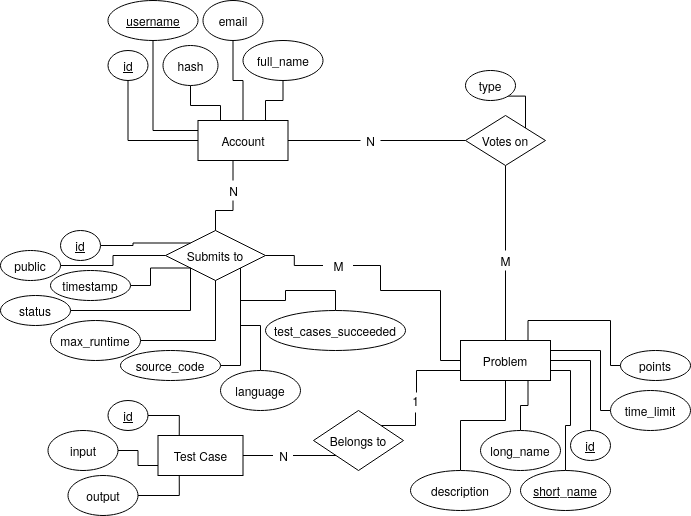
\includegraphics[width=0.9\textwidth]{database-schema}
	\caption{Databasstruktur}\label{dbschema}
\end{figure}

Sedan skapades denna struktur i en faktisk databas. Värt att notera är att
``type'', tillhörande ``Votes on'', är en \textit{enumeration} med de möjliga
värdena ``upp'' och ``ner''. ``status'', tillhörande ``Submits to'' motsvarar
\mintinline[bgcolor=codebg]{sh}|Status| i \coderef{status-enum}.

\subsubsection{Webbserver}
\label{webbserver}

Som tidigare nämnt valdes ramverket Sapper till att bygga webbservern. Sapper är
speciellt i och med att HTML:en genereras av JavaScript, och detta sker både på
servern och i webbläsaren beroende på situation. När en användare först går in
på sidan genereras allt på servern. I andra fall, som när användaren går till en
annan del av sidan, används AJAX för att hämta eventuell data och nödvändig HTML
genereras i webbläsaren och ersätter endast de delar av sidan som ändras.

\paragraph{Sessioner}

För att webbapplikationen ska erbjuda en användarvänlig upplevelse bestämdes att
spara en användares ``session'' efter att denna loggat in.

För att åstadkomma detta på ett säkert sätt används oftast en ``sessionskaka''.
I användarens webbläsare sparas ett unikt identifikationsnummer och på
webbservern en tabell med dessa identifikationsnummer kopplade till data om det
inloggade kontot.

% TODO: snabbgenomgång om feistelkrypto?

För att undvika att behöva spara detta i webbservern valdes istället att spara
denna data i kakan. Men för att göra detta säkert krypterades kakan med det
symmetriska ``Feistelkryptot''. Detta gör det omöjligt för en illvillig
användare att både läsa datan i kakan och försöka ändra datan i den så länge
denne inte har tillgång till de hemliga nycklarna som används vid kryptering och
avkryptering. Utöver själva datan krypteras även en slumpad uppsättning bytes
och tiden vid kryptering. På detta sätt kan en session ``ta slut'' om användaren
exempelvis lämnar datorn. Dessutom resulterar samma sessionsdata i olika
krypterade kakor olika gånger.

Nedan följer funktionen som används för att kryptera kakorna.

\begin{listing}[H]
	\caption{Kryptering av kakor}
	\begin{minted}[bgcolor=codebg,autogobble,tabsize=4]{js}
		export function encrypt(token, keys, randSize) {
			let rand = crypto.randomBytes(randSize);
			let date = Date.now().toString();
			let payload = Buffer.from(JSON.stringify(token));

			let data = Buffer.concat([
				rand,
				Buffer.from(date),
				Buffer.from([0]),
				payload,
			]);

			if (data.length % 2)
				data = Buffer.concat([data, Buffer.from([0])]);

			let l = data.slice(0, data.length / 2);
			let r = data.slice(data.length / 2, data.length);
			for (let key of keys.slice(0, keys.length - 1)) {
				let nl = r;
				let f = crypto.createHash("sha512")
					.update(Buffer.concat([Buffer.from(key), r]))
					.digest();
				let nr = l.map((byte, i) => byte ^ f[i % f.length]);
				l = nl;
				r = nr;
			}

			let f = crypto.createHash("sha512")
				.update(Buffer.concat(
					[Buffer.from(keys[keys.length - 1]), r]
				))
				.digest();
			l = l.map((byte, i) => byte ^ f[i % f.length]);

			return Buffer.concat([rand, l, r]).toString("hex");
		}
	\end{minted}
\end{listing}

Avkrypteringen fungerar likadant, fast bakvänt.

\paragraph{Ändpunkter}

I ett projekt gjort med Sapper placeras alla ändpunkter webbservern ska
tillgängliggöra i separata filer. Beroende på vilka HTTP-förfrågningsmetoder som
ska finnas tillgängliga på ändpunkten exporterar filen funktioner med
motsvarande namn. (Alltså ``get'', ``post'', ``head'', osv). Ändpunkter ges
filänden \mintinline[bgcolor=codebg]{sh}|.json.js|, men
\mintinline[bgcolor=codebg]{sh}|.js| finns ej med i ändpunktens namn när
klienten skickar en förfrågan. Dessa filer placeras i mappen
\mintinline[bgcolor=codebg]{sh}|/src/routes/| som ligger i projektets rot.

Om exempelvis filen \mintinline[bgcolor=codebg]{sh}|src/routes/foo/bar.json.js|
exporterar funktionen \mintinline[bgcolor=codebg]{sh}|get| kan webbservern ta
emot en \textit{get}-förfrågan på
\mintinline[bgcolor=codebg]{sh}|/foo/bar.json|.

Funktionerna anropas när någon skickar en HTTP-förfrågan till ändpunkten. I
funktionerna tillgängliggörs två parametrar:
\mintinline[bgcolor=codebg]{sh}|req| och \mintinline[bgcolor=codebg]{sh}|res|.
\mintinline[bgcolor=codebg]{sh}|req| beskriver information om förfrågan som
skickades och \mintinline[bgcolor=codebg]{sh}|res| används för att skicka
tillbaka ett svar.

Nedan följer ett exemepl på en ändpunkt som implementerades i detta projekt.
Filen heter \mintinline[bgcolor=codebg]{sh}|src/routes/login.json.js| och definierar en ändpunkt som
används för att logga in ett konto och därmed skapa en session.

\begin{listing}[H]
	\caption{Inloggningsändpunkten}
	\begin{minted}[bgcolor=codebg,autogobble,tabsize=4]{js}
		import bcrypt from "bcrypt";
		import database from "../database";
		import * as responses from "../responses";

		export async function post(req, res) {
			const { username, password } = req.body;

			if (!username || !password)
				return responses.missingParam(res, "username/password");

			const result = await database.query(
				"SELECT id, hash FROM account WHERE username = ?",
				username,
			);

			if (result.length == 0)
				return responses.invalid(res, "username");

			const { id, hash } = result[0];

			const correctPassword = await bcrypt.compare(password, hash);

			if (!correctPassword)
				return responses.invalid(res, "password");

			req.token = { id };

			res.send({ msg: "Logged in" });
		}
	\end{minted}
\end{listing}

Först kontrolleras att förfrågan är korrekt, alltså att både ett användarnamn
och ett lösenord har skickats med. Sedan hämtas kontots unika
identifikationsnummer och lösenordshash från databasen. Efter det kontrolleras
att ett konto hittades och att lösenordet matchar med hashen i databasen. För
detta används algoritmen \textit{bcrypt} från ett externt bibliotek.

Slutligen sparas kontots identifikationsnummer i
\mintinline[bgcolor=codebg]{sh}|req.token|. Detta
kommer sedan automatisk krypteras och skickas med som en kaka innan servern
svarar klienten.

Ett annat exempel på ändpunkt är den där information om en specifik inlämning
hämtas. Filen heter \mintinline[bgcolor=codebg]{sh}|routes/submissions/[submission]/index.json.js|. Att
rutten har en del med hakparanteser i sig leder till att ändpunkten blir
dynamisk och \mintinline[bgcolor=codebg]{sh}|/submissions/<vad som helst>.json| kan anropas. Notera även
att \mintinline[bgcolor=codebg]{sh}|/index| ej måste finnas med i förfrågan.

\begin{listing}[H]
	\caption{Inlämningshämtningsändpunkten}
	\begin{minted}[bgcolor=codebg,autogobble,tabsize=4,linenos]{js}
		import database from "../../../database";
		import * as responses from "../../../responses";
		import depthify from "../../../depthify";
		import { langName } from "../../../judge";

		export async function get(req, res) {
			const { submission } = req.params;
			const accountId = req.token ? req.token.id : -1;
			const result = await database.query(
				`SELECT
					username AS "submitter.username",
					full_name AS "submitter.fullName",
					problem.short_name AS "problem.shortName",
					problem.long_name AS "problem.longName",
					public, timestamp, lang, source, status,
					max_runtime_ms AS maxRuntime,
					test_cases_succeeded AS "testCases.succeeded",
					COUNT(test_case.id) AS "testCases.total",
					account_id = ? AS requesterIsOwner
				FROM submission, problem, account, test_case
				WHERE submission.id = ?
				AND submission.problem_id = problem.id
				AND submission.account_id = account.id
				AND test_case.problem_id = problem.id
				GROUP BY submission.id`,
				[accountId, submission]
			);

			if (result.length === 0) return res.status(404).send({
				msg: "Unknown submission"
			});

			if (!(result[0].public || result[0].requesterIsOwner))
				return res.status(403).send({
					msg: "You dont have access to this submission"
				});

			result[0].lang = langName(result[0].lang);
			res.send(depthify({ ...result[0] }));
		}
	\end{minted}
\end{listing}

Majoriteten av denna ändpunkt är ett SQL-query. Notera att
\mintinline[bgcolor=codebg]{sh}|req.token.id| används. Detta är från början inte
en del av förfrågan, eftersom klienten inte känner till sitt
identifikationsnummer, utan ``sätts in'' av en annan funktion innan denna
anropas.

\subsubsection{Webbsida}

Sapper, som använts till webbservern, är sammankopplat med webbsideramverket
``Svelte''. Detta medger att webbsidan måste vara byggd med Svelte. Sapper kan
också ses som en utbyggnad av Svelte.

Nackdelen med att använda AJAX \--- \underline{a}synchronous
\underline{J}avaScript \underline{a}nd \underline{X}ML, asynkron JavaScript och
XML är att det kan göra webbsidors initiala laddtid långsammare. Detta för att
webbläsaren först hämtar all HTML, CSS och JavaScript, sedan körs ett skript som
får webbläsaren att fråga servern igen om data som behövs för att visa sidan.

Sapper löser detta genom att en \textit{rutt} kan definiera en speciell funktion
som hämtar den data som krävs för att visa sidan. Om en användare går till en
sådan rutt direkt körs denna funktion redan på servern. Om funktionen hämtar
data från samma server görs detta med ett vanligt funktionsanrop. Denna data
skickas då med samtidigt som resten av sidan skickas.

Men om användaren går från en rutt till en annan genom att följa en hyperlänk
behöver inte hela sidan ladda om, utan Sapper ser till att endast den nya
HTML:en, CSS:en, JavaScripten och datan som krävs hämtas från servern. I detta
fall körs den omtalade funktionen på webbläsaren. Samma funktion kan alltså både
köras på servern och i webbläsaren.

Svelte i sig är ett ramverk som låter utvecklaren dela upp webbsidan i olika
komponenter som hanterar sig själva. En komponent består av tre huvuddelar:

\begin{itemize}
	\item HTML-liknande kod som översätts till JavaScript som sedan genererar
		riktigt HTML.
	\item CSS-stiltaggar som ändrar utseendet på HTML:en i just den egna
		komponenten. Stiltaggarna i olika komponenter hindras alltså från att
		``krocka'' med varandra.
	\item JavaScript som påverkar vad HTML:en innehåller, hämtar data, och gör
		webbsidan interaktiv.
\end{itemize}

Rutterna på hemsidan sparas också i \mintinline[bgcolor=codebg]{sh}|src/routes/|
och har filändelsen \mintinline[bgcolor=codebg]{sh}|.svelte|, men denna är ej
med i rutten webbläsaren hämtar.

Ett förenklat exempel på en sådan rutt i detta projekt är
\mintinline[bgcolor=codebg]{sh}|src/routes/login.svelte|, som alltså koms åt av
webbläsaren på \mintinline[bgcolor=codebg]{sh}|/login| som följer nedan:

\begin{listing}[H]
	\caption{Förenkling av rutten \mintinline[bgcolor=codebg]{sh}|/login|}
	\begin{minted}[bgcolor=codebg,autogobble,tabsize=4,linenos]{html}
		<style>
			.error {
				color: red;
			}
		</style>
		<script>
			import { goto } from "@sapper/app";
			import { slide } from "svelte/transition";

			let errors = [];
			let username = "";
			let password = "";

			async function submit() {
				msgs = [];

				if (!username)
					return errors = ["Missing username"];
				if (!password)
					return errors = ["Missing password"];

				const res = await fetch("/login.json", {
					method: "post",
					headers: {
						"Content-Type": "application/json",
					},
					body: JSON.stringify({
						username,
						password,
					}),
				});
				const json = await res.json();

				if (res.status === 200) goto("/");
				else errors = [...errors, json.msg];
			}
		</script>
		<input id="username" type="text" bind:value={username} />
		<input id="password" type="password" bind:value={password} />
		<button on:click={submit}>Log in</button>
		{#each errors as error (error)}
			<p transition:slide class="error">{error}</p>
		{/each}
	\end{minted}
\end{listing}

Värt att notera är
\mintinline[bgcolor=codebg]{css}|bind:value={/*...*/}|-syntaxen. Detta är
Svelte-specifikt och ``binder'' ihop ett värde med en variabel. I det här fallet
binds variabeln \mintinline[bgcolor=codebg]{js}|username| samman med texten som
står i inputfältet på webbsidan. Detta medger att om variabeln ändras från
skriptet så ändras texten i fältet och när användaren ändrar texten i fältet
ändras även variabeln.

Längst ner används sveltes \mintinline[bgcolor=codebg]{sh}|#each|-syntax. Detta
efterliknar en for-loop då detta exempel producerar ett paragrafelement för
varje värde i listan \mintinline[bgcolor=codebg]{js}|errors|. Dessutom markeras
elementen att använda övergången \mintinline[bgcolor=codebg]{js}|slide|, som är
inbyggd Svelte. Dessa inbyggda övergångar underlättar att skapa en mer
rörlig och animerad webbsida.

Notera även att funktionen \mintinline[bgcolor=codebg]{js}|submit| anropas när
knappen trycks av användaren och att denna skickar en HTTP-förfrågan till
servern. Dataformatet som används är även här JSON.

\section{Resultat}

Resultatet blev i huvudsak som planerat. Användares program exekveras på ett
säkert sätt, deras programs exekveringstid mäts på ett (relativt) konsekvent
sätt och användarupplevelsen är både säker och tillfredsställande.

Webbsidan är i ett adekvat fungerande skick. Dessa funktioner har
implementerats:

\begin{itemize}
	\item Registrering av konto
	\item Inloggning med konto
	\item Topplista, där konton rangordnas efter antal insamlade ``poäng''
	\item Visning av konto
	\item Lista av problem
	\item Visning av specifikt problem
	\item Röstning på problem
	\item Uppvisning av information om inlämningar till specifikt problem
	\item Inlämning till problem
	\item Bedömning av inlämning
	\item Lista av användarens egna inlämningar
	\item Möjlighet att markera inlämning som publik
	\item Visning av specifik inlämning (resultat + källkod)
	\item Kontoinställningar
	\item Möjlighet att skapa problem
\end{itemize}

Språk som går att skapa lösningar och skicka in är C och C++. Domaren har
kodmässigt möjlighet att bedöma samtliga kompilerade språk, men ytterligare
konfiguration skulle behöva tilläggas.

Nedan följer ett fåtal bilder av den utvecklade produkten.

\begin{figure}[H]
	\centering
	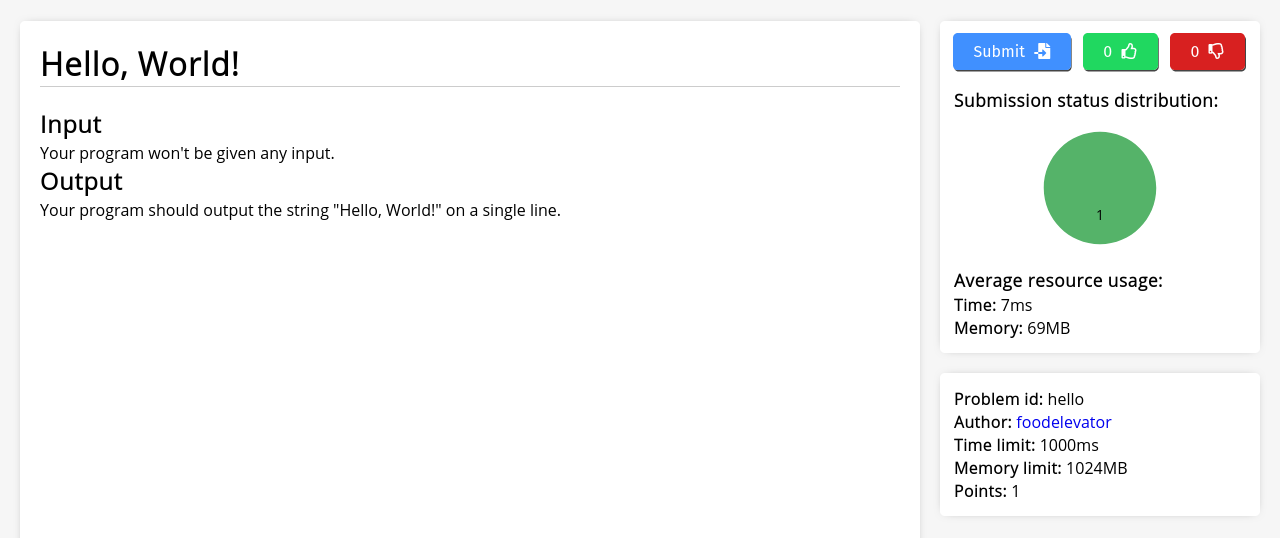
\includegraphics[width=1\textwidth]{problem}
	\caption{Visning av problem}
\end{figure}

\begin{figure}[H]
	\centering
	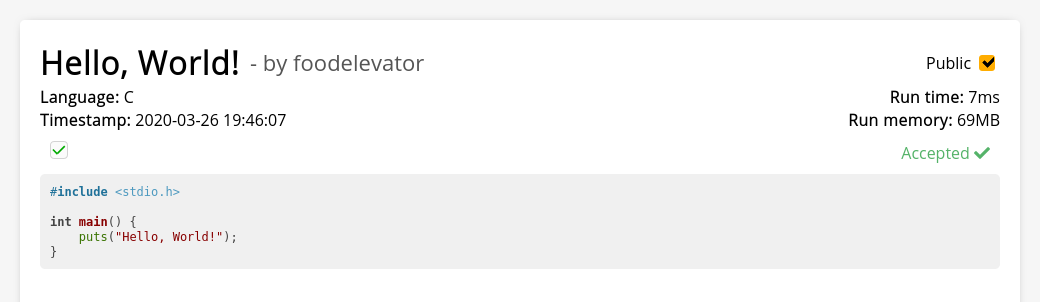
\includegraphics[width=1\textwidth]{submission}
	\caption{Visning av inlämning}
\end{figure}

\begin{figure}[H]
	\centering
	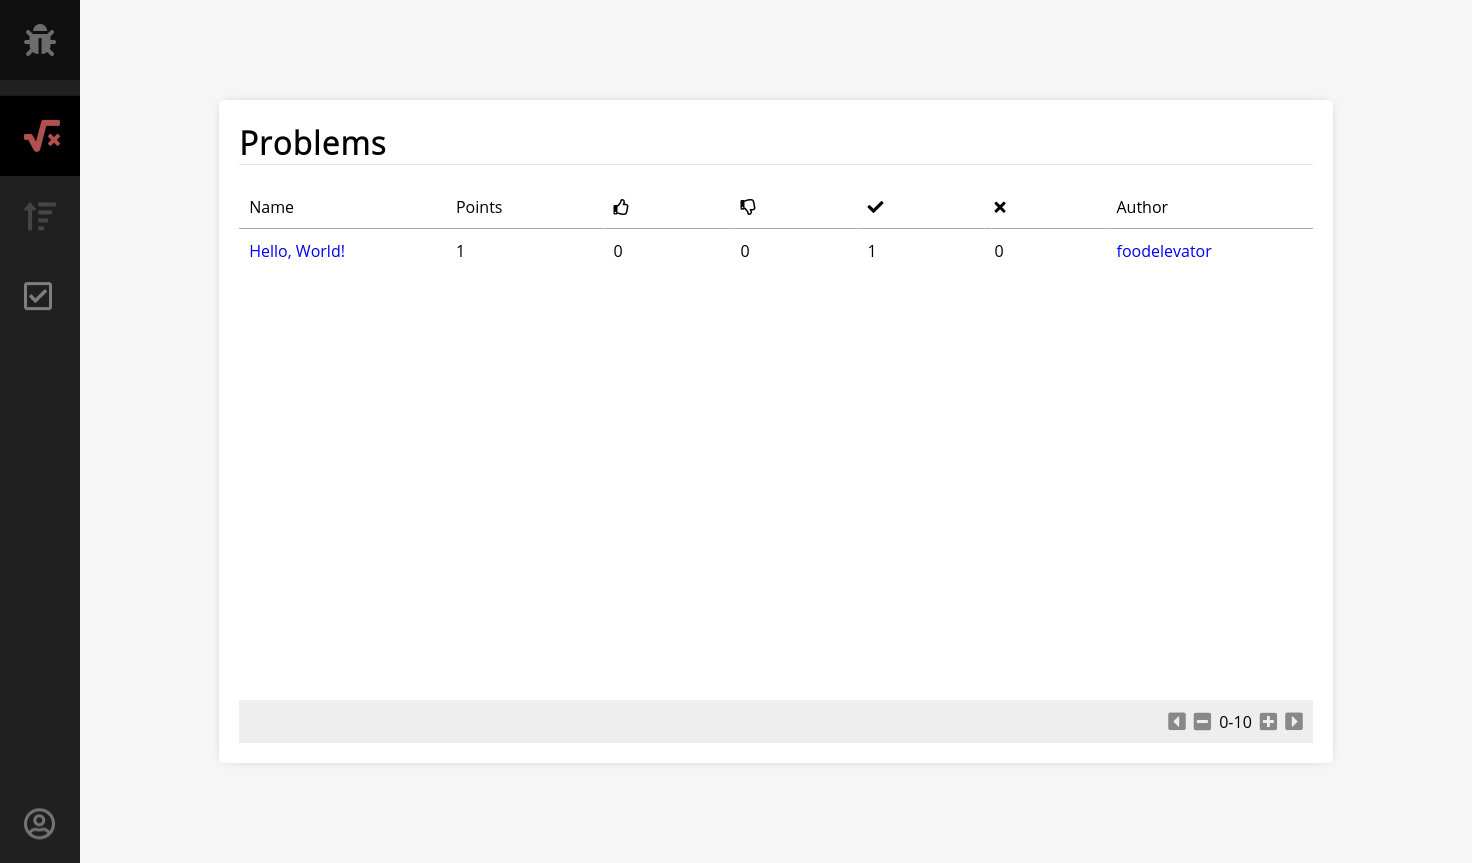
\includegraphics[width=1\textwidth]{problem-list}
	\caption{Lista av problem}
\end{figure}

\begin{figure}[H]
	\centering
	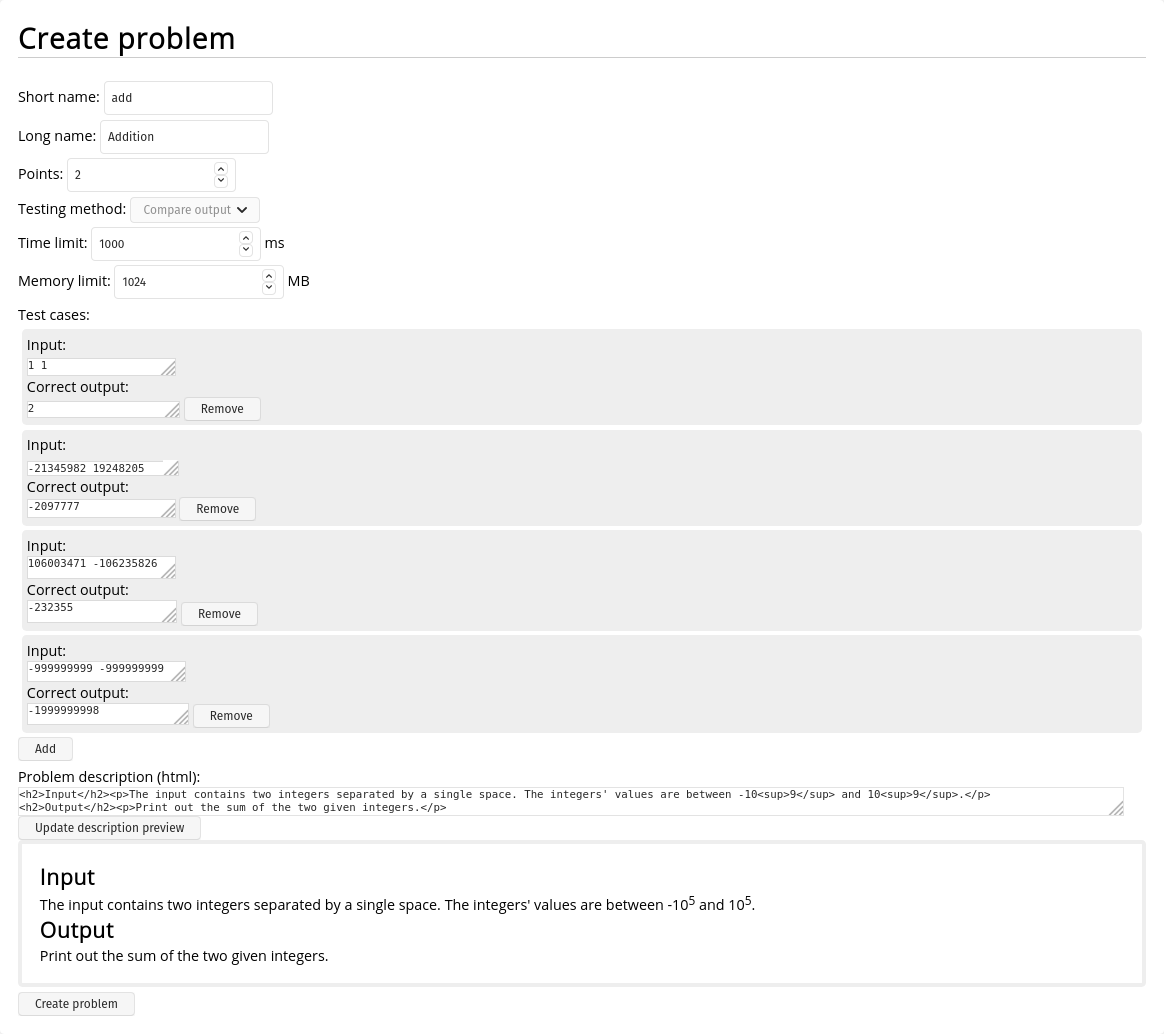
\includegraphics[width=1\textwidth]{create-problem}
	\caption{Skapandet av nytt problem}
\end{figure}

\section{Diskussion / Slutsatser}

I sin helhet anser jag att projektet blev lyckat. Tyvärr blev webbsidan lite
bristfällig på vissa områden, som t.ex. första sidan som visas. Denna är i
princip helt tom.

\subsection{Hur exekveras opålitlig kod på ett säkert sätt?}

Med användningen av chroot, ändring till en annan användare samt
brandväggsregeln som förhindrar användaren från att nå internet \underline{bör}
exekveringen ske säkert. Men med de flesta andra säkerhetsriskerna är det svårt
att vara \underline{helt} garanterad om att detta stämmer.

Mig veterligen finns dock inga säkerhetshål kvar.

\subsection{Hur mäts ett programs körningstid samt minnesallokeringsmängd på
	ett konsekvent sätt?}

Som beskrivet tidigare i rapporten är det viktigt att inte exekvera för många
användarprogram samtidigt, samt att andra processer inte ``stjäl'' användarnas
programs proccessortid.

Ett stort problem är dock att denna domare mäter den riktiga tid som passerar
från att användarens program startas till att den avslutas. Istället går det
även att mäta just tiden som spenderats till att exekvera ett visst program.
Från vad jag hittat så verkar det endast möjligt att mäta detta för den
nuvaranda processen eller för samtilga ``barnprocesser'' samtidigt (med
syscallet \textit{getrusage}). Det skulle möjligvis gå att göra detta från
\textit{executor}, men då skulle ej \textit{execve} kunna användas, eftersom
funktionen aldrig returnerar. Det är därför inte möjligt att helt enkelt mäta
tiden det tog efter att användarens program exekveras klart.

Alltså mäts körningstiden, men inte nödvändigvis helt konsekvent.

Mätning av minnesallokeringsmängden hann jag tyvärr inte implementera. Det
verkar som att två alternativ finns: kontrollera detta konstant, om och om igen,
eller att använda \textit{getrusage}, vilket bland annat ger ``det maximala
antalet kilobytes fysiskt minne programmet använde samtidigt''. Då stöter man
dock på samma problem som med att mäta tiden.

\subsection{
	Hur implementeras en både tillfredsställande och säker användarupplevelse?
}

Sessioner är en bra kompromiss mellan säkerhet och smidighet för användaren. Att
inte alls ha sessioner och istället kräva användarens lösenord varje gång denna
vill göra något är på vissa sätt ett säkrare alternativ. Det stora problemet med
detta är dock att det webbsidan blir väldigt jobbig att använda.

En populär lösning på detta är att spara data om användarens session på i en
databas och spara ett ID in till databasen i en kaka i webbläsaren.

Egentligen är denna lösning lite säkrare än det som implementerades i detta
projekt, eftersom det låter webbservern aktivt invalidera sessioner om i fall
det skulle krävas. Den enda egentliga fördelen med metoden i projektet är att
den är lite snabbare, eftersom den inte kräver ett databasuppslag. Anledningen
till att jag valde denna implementation var främst för att det verkade roligt
att göra.

En annan populär lösning är att använda s.k. JSON Web Tokens. Dessa fungerar
väldigt likt det jag själv implementerade, med den huvudsakliga skillnaden att
de vanligtvis inte krypteras. Samtidigt ville jag inte att användaren skulle få
veta vad som sparas i dess session. Det största biblioteket,
\textit{jsonwebtoken}, till node har inte stöd för kryptering och när jag
bestämde mig för detta kände jag inte till att ett annat bibliotek fanns, som
har stöd för krypering.

\section{Referenser}

\begin{itemize}
	\item Competetive Programming, Wikipedia \\
		\url{https://en.wikipedia.org/wiki/Competitive_programming}
	\item International Collegiate Programming COntest, Wikipedia \\
		\url{https://en.wikipedia.org/wiki/International_Collegiate_Programming_Contest}
	\item Programmeringsolymnpiaden \url{https://www.progolymp.se/}
	\item Kattis öppna problemsamlig \url{https://open.kattis.com/}
	\item Codeforces \url{https://codeforces.com/}
	\item Dockers dokumentation \url{https://docs.docker.com/get-docker/}
	\item GCC \url{https://gcc.gnu.org/}
	\item Manualen för chroot \\
		\url{http://man7.org/linux/man-pages/man2/chroot.2.html}
	\item Säkerhet runt chroot \\
		\url{https://filippo.io/escaping-a-chroot-jail-slash-1/}
	\item Manualen för iptables \\
		\url{https://linux.die.net/man/8/iptables}
	\item Rusts webbsida \url{https://rust-lang.org}
	\item Rusts standardbibioteks dokumentation \\
		\url{https://doc.rust-lang.org/std/}
	\item Serdes dokumentation \url{https://docs.serde.rs/serde/}
	\item Trådpool \url{https://en.wikipedia.org/wiki/Thread_pool}
	\item Node.js dokumentation \\
		\url{https://nodejs.org/dist/latest-v13.x/docs/api/}
	\item Expressjs dokumentation \url{https://expressjs.com/en/4x/api.html}
	\item Sappers dokumentation \url{https://sapper.svelte.dev/}
	\item Feistelkrypto \url{https://en.wikipedia.org/wiki/Feistel_cipher} och
		\\ \url{https://www.youtube.com/watch?v=FGhj3CGxl8I}
	\item Guide för getrusage
		\url{https://www.gnu.org/software/libc/manual/html_node/Resource-Usage.html}
	\item Manualen för getrusage
		\url {https://linux.die.net/man/2/getrusage}
	\item JSON Web Tokens \url{https://jwt.io}
\end{itemize}

\section{Bilagor}

\listoffigures{}

\listoflistings{}

\end{document}
